% LaTeX source for ``การเรียนรู้ของเครื่องสำหรับเคมีควอนตัม (Machine Learning for Quantum Chemistry)''
% Copyright (c) 2022 รังสิมันต์ เกษแก้ว (Rangsiman Ketkaew).

% License: Creative Commons Attribution-NonCommercial-NoDerivatives 4.0 International (CC BY-NC-ND 4.0)
% https://creativecommons.org/licenses/by-nc-nd/4.0/

\chapter{คุณสมบัติเชิงอิเล็กทรอนิกส์ของโมเลกุล}
\label{ch:el_prop}

เนื้อหาในบทนี้จะเกี่ยวกับทฤษฎีของคุณสมบัติเชิงอิเล็กทรอนิกส์ (Electronic Properties) ของโมเลกุลซึ่งผู้เขียนแล้วคิดว่าเป็นสิ่งที่สำคัญมาก
นั่นก็เพราะว่าการที่เราต้องการจะเชื่อมโยง ML และเคมีควอนตัมเข้าด้วยกันนั้นเราจะต้องเข้าใจถึงคุณสมบัติของโมเลกุลที่เราจะศึกษาเสียก่อน

โมเลกุลเป็นหน่วยพื้นฐานของสิ่งต่าง ๆ รอบตัวเรา โมเลกุลก็คือกลุ่มของอะตอมหลาย ๆ อะตอมมารวมกัน และในอะตอมนั้นเราสนใจอิเล็กตรอนเป็นพิเศษ
ในวิชาควอนตัมนั้นเราจะอธิบายพฤติกรรมของโมเลกุลโดยมุ่งเน้นไปที่อิเล็กตรอนซึ่งสามารถที่จะถูกอธิบายได้ด้วยฟังก์ชันทางคณิตศาสตร์ที่เรียกว่า 
\enquote{\textit{ฟังก์ชันคลื่น (Wavefunction)}} ซึ่ง Wavefunction นั้นจริง ๆ แล้วเป็นแนวคิดและไม่มีรูปร่างหน้าตาหรือการนิยามแบบที่%
แน่นอนหรือตายตัว โดยหนึ่งในสมการที่โด่งดังที่สุดสมการหนึ่งของวงการวิทยาศาสตร์นั่นคือสมการชโรดิงเงอร์ (Schrödinger Equation)%
\autocite{schrodinger1926} ซึ่งถูกพัฒนาโดยศาสตราจารย์ Erwin Schrödinger โดยบทความงานวิจัยชิ้นแรกของสมการชโรดิงเงอร์ถูกตีพิมพ์%
ในเดือนมกราคม ปี ค.ศ. 1926\footnote{ศาสตราจารย์ Erwin Schrödinger นักฟิสิกส์เชื้อสายออสเตรีย-ไอริช ได้รับรางวัลโนเบลสาขาฟิสิกส์ 
ค.ศ. 1933 ร่วมกับศาสตราจารย์ Paul Dirac (อ้างอิง \url{https://www.nobelprize.org/prizes/physics/1933/summary/})} 
โดยสมการชโรดิงเงอร์ถูกนำมาใช้ในการศึกษาระบบทางกลศาสตร์ควอนตัมซึ่งการแก้สมการชโรดิงเงอร์ได้นั้นจะทำให้ได้มาซึ่งสมการคณิตศาสตร์ที่อธิบาย 
Wavefunction

\begin{figure}[H]
    \centering
    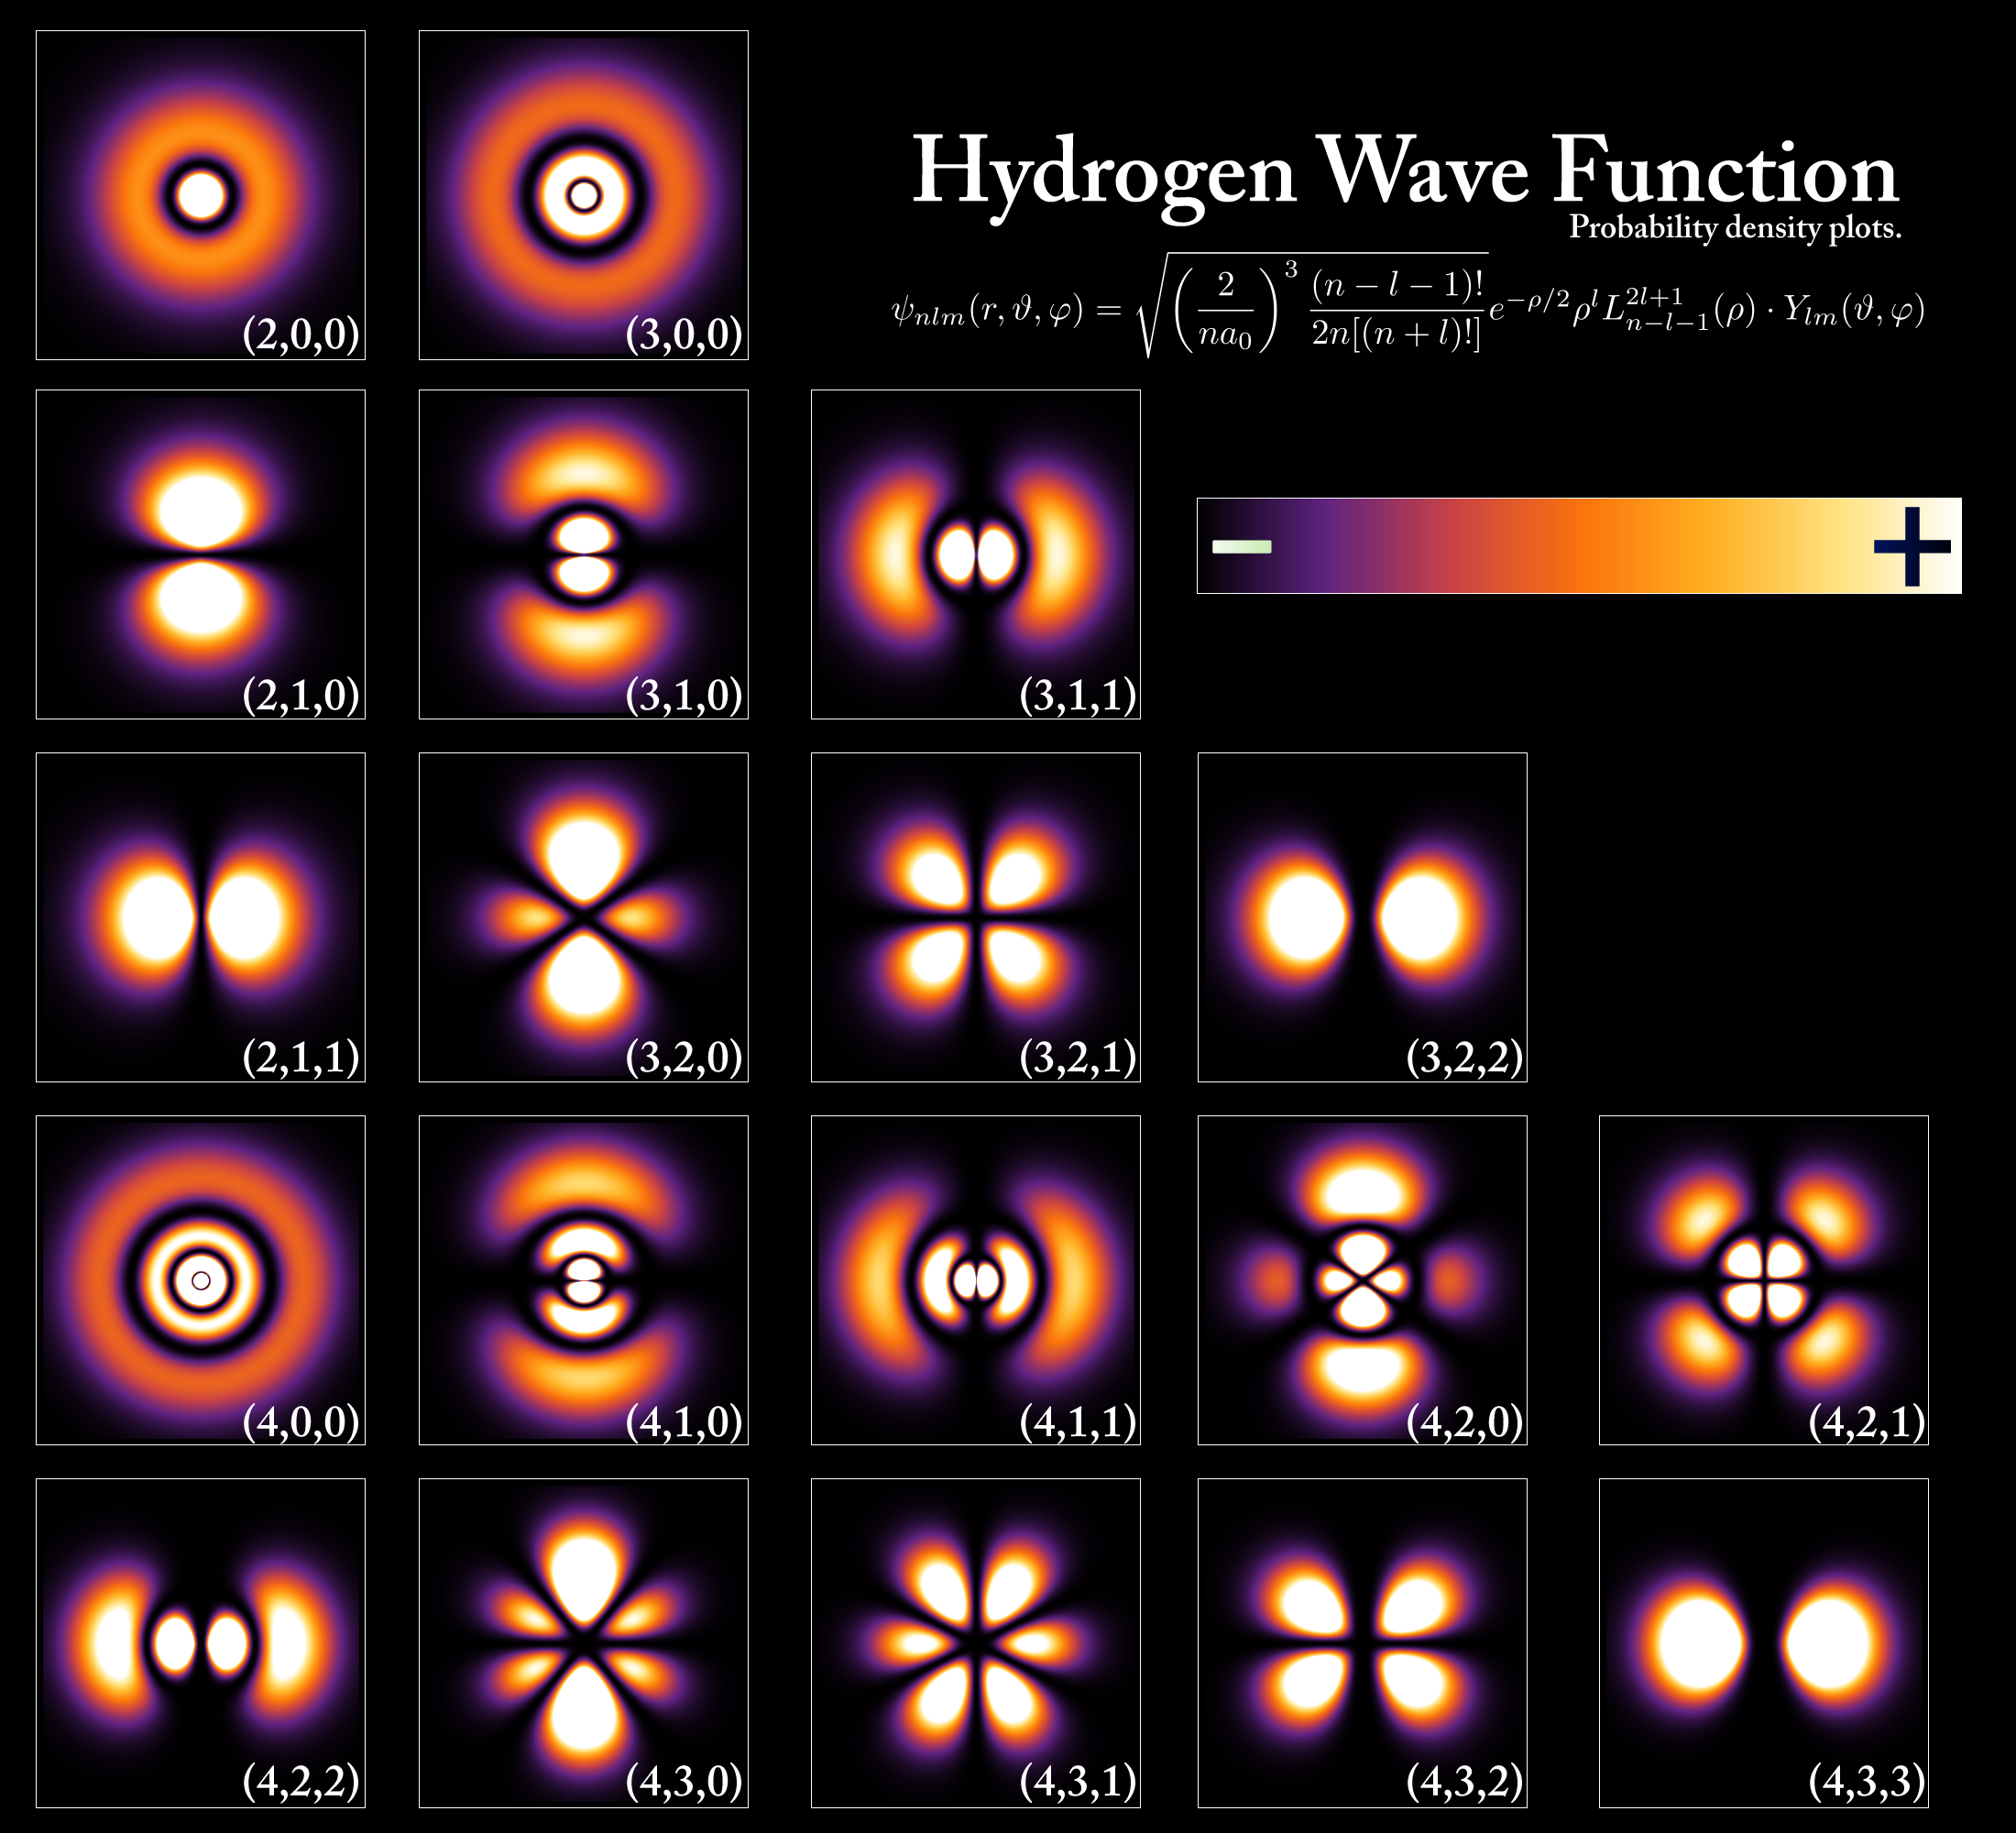
\includegraphics[width=0.8\linewidth]{fig/hydrogen_density_plots.png}
    \caption{แบบจำลองของออร์บิทัลเชิงอะตอม (Atomic Orbitals) ของอิเล็กตรอนของอะตอมไฮโดรเจนที่ระดับพลังงานที่แตกต่างกัน
    โดยความเข้มของสีที่ไฮไลท์บ่งบอกถึงโอกาสที่จะพบอิเล็กตรอน ณ ตำแหน่งนั้น 
    (เครดิตภาพ: \url{https://en.wikipedia.org/wiki/Atomic_orbital})}
    \label{fig:hydrogen_density}
\end{figure}

สมการชโรดิงเงอร์สามารถแบ่งออกได้เป็นสองแบบคือแบบที่ไม่ขึ้นกับเวลาและแบบที่ขึ้นกับเวลา ดังนี้\autocite{szabo1996,cramer2004,jensen2017}

\noindent $\bullet$ \textbf{1. Time-dependent Schrödinger Equation}

\begin{equation}\label{eq:tdse}
    i \hbar \frac{d}{d t} \ket{\Psi(t)} = \hat{H} \ket{\Psi(t)}
\end{equation}

\noindent $\bullet$ \textbf{2. Time-independent Schrödinger Equation}

\begin{equation}\label{eq:tise}
    \hat{H}\ket{\Psi} = E \ket{\Psi}
\end{equation}

โดย Wavefunction ($\Psi(t)$) ที่เป็น Eigenfunction นั้นจะบรรจุข้อมูลเชิงอิเล็กทรอนิกส์ทุกอย่างเกี่ยวกับระบบของเราเอาไว้ ซึ่งระบบใน%
ที่นี้ก็คือโมเลกุล โดยสมการข้างต้นเป็นการคำนวณหาพลังงานของระบบโดยใช้ Hamiltonian Operator ($\hat{H}$) ซึ่งเป็น Operator 
ที่สอดคล้องกับพลังงาน ซึ่งจริง ๆ แล้ว Eigenvalue ของสมการข้างต้น (สมการที่ \ref{eq:tdse} และ \ref{eq:tise}) จะเป็นคุณสมบัติ%
ของโมเลกุลอะไรก็ได้ ตราบใดที่เราใช้ Operator ที่สอดคล้องกับคุณสมบัตินั้น ๆ 

%--------------------------
\section{แฮมิลโทเนียน}
\label{sec:hamiltonian}
%--------------------------

Hamiltonian เป็นสิ่งที่สำคัญมากในเคมีควอนตัมเพราะเปรียบเสมือนเป็นกุญแจที่สามารถไขรหัสหาคำตอบหรือความลับจาก Wavefunction ได้
โดย Hamiltonian Operator ที่เรานำมาใช้งานนั้นจริง ๆ แล้วก็คือ Operator สำหรับการหาพลังงานรวมนั่นเอง โดยเป็นผลรวมของ Operator 
พลังงานจลน์และพลังงานศักย์
\idxen{Operator}
\idxboth{แฮมิลโทเนียน}{Hamiltonian}

\begin{equation}\label{eq:hamiltonian}
    \hat{H} = \hat{T} + \hat{V}
\end{equation}

\noindent โดยที่พลังงานจลน์นั้นสามารถเขียนให้อยู่ในรูปของ Momentum Operator ได้โดยพิสูจน์จากพลังงานจลน์ในกรณีแบบดั้งเดิม ดังนี้
\idxboth{โมเมนตัม}{Momentum}
\idxboth{พลังงานจลน์}{Kinetic Energy}

\begin{align}
    T &= \frac{1}{2}mv^{2}_{x} \\
      &= \frac{(mv_{x})^{2}}{2m}
\end{align}

\noindent ทำการจัดรูปใหม่แล้วทำการแทนเทอม $mv_{x}$ ด้วย Momentum Opeator $-ih\frac{d}{dx}$ จะได้ Operator ใหม่ดังนี้

\begin{equation}
    \hat{T} = -\frac{\hbar^{2}}{2m}\frac{d^{2}}{dx^{2}}
\end{equation}

สำหรับพลังงานศักย์นั้นตรงไปตรงมา นั่นคือเราสามารถเขียนพลังงานศักย์ในทางควอนตัมได้แบบเดียวกับกรณีกลศาสตร์ดั้งเดิมได้เลย ดังนี้
\idxboth{พลังงานศักย์}{Potential Energy}

\begin{equation}
    \hat{V} = V(x)
\end{equation}

เมื่อเรานำ Operator ของทั้งสองพลังงานมารวมกันเราจะได้ Hamiltonian Operator ดังนี้

\begin{equation}
    \hat{H} = -\frac{\hbar^{2}}{2m}\frac{d^{2}}{dx^{2}} + V(x)
\end{equation}

ลำดับต่อมาคือเราจะมาทำการพิจารณาพลังงานศักย์กันก่อนเพราะว่าไม่ซับซ้อนเหมือนกับกรณีของพลังงานจลน์ โดยพลังงานศักย์ที่เราจะพิจารณาก็คือ%
พลังงานงานศักย์คูลอมบ์ (Coulomb Potential Energy หรือ Operator นั่นเอง) โดยมีสมการดังต่อไปนี้
\idxboth{พลังงานงานศักย์!พลังงานคูลอมบ์}{Potential Energy!Coulomb Energy}

\begin{equation}
    E_{q_{1}q_{2}} = q_{1}\frac{q_{2}}{4\pi\epsilon_{0}|\boldmath{R}|}
\end{equation}

โดยเมื่อเราพิจารณาระบบง่าย ๆ เช่น อะตอมไฮโดรเจนซึ่งมี 1 อิเล็กตรอนและ 1 นิวเคลียส แล้วกำหนดจุดกำเนิด (Origin Point) ซึ่งมีระยะห่าง%
จากอิเล็กตรอนเท่ากับ $\boldmath{r}$ หน่วยและมีระยะห่างจากนิวเคลียสเท่ากับ $\boldmath{R}$ หน่วย จะได้ว่าระยะห่างระหว่างอิเล็กตรอนและ%
นิวเคลียวคือ $\boldmath{r}-\boldmath{R}$ หน่วย ดังนั้นเราสามารถเขียน Hamiltonian Operator ได้ดังนี้

\begin{align}\label{eq:hamiltonian_hydrogen}
    \hat{H} =& -\frac{\hbar^{2}}{2M} \left( \pdv[2]{X} + \pdv[2]{Y} + \pdv[2]{Z} \right) 
              -\frac{\hbar^{2}}{2m} \left( \pdv[2]{x} + \pdv[2]{y} + \pdv[2]{z} \right) \nonumber \\
             &-\frac{1}{4\pi\epsilon_{0}}\frac{e^{2}}{\boldmath{r}-\boldmath{R}}
\end{align}

\noindent โดยเราสามารถใช้สัญลักษณ์ $\nabla^{2}$ หรือ Laplace Operator ($\nabla$ อ่านว่า Nabla) ซึ่งเป็นอนุพันธ์อันดับที่สอง%
ของพลังงานจลน์ของนิวเคลียส (เทอมแรก) และของพลังงานจลน์ของอิเล็กตรอน (เทอมที่สอง) ของสมการที่ \ref{eq:hamiltonian_hydrogen} 
โดยสามารถเขียนสมการใหม่ได้ดังนี้

\begin{equation}\label{eq:hamiltonian_reduced}
    \hat{H} = -\frac{\hbar^{2}}{2M} \nabla^{2}_{\boldmath{R}} - \frac{\hbar^{2}}{2m} \nabla^{2}_{\boldmath{r}}
              -\frac{1}{4\pi\epsilon_{0}}\frac{e^{2}}{\boldmath{r}-\boldmath{R}}
\end{equation}

ถึงแม้ว่าสมการที่ \ref{eq:hamiltonian_reduced} มีความเรียบง่ายแล้วแต่ว่าในเคมีควอนตัมนั้นเราจะไม่ได้ใช้สมการของ Operator ที่อยู่ในหน่วย
SI (SI Units) แต่เราใช้หน่วยอะตอม (Atomic Units) แทน ซึ่งเมื่อเราเขียนสมการในรูปของ Atomic Units แล้วจะได้สมการที่เรียบง่ายกว่าเดิม
ดังนี้

\begin{equation}\label{eq:hamiltonian_reduced}
    \hat{H} = -\frac{1}{2M} \nabla^{2}_{\boldmath{R}} - \frac{1}{2} \nabla^{2}_{\boldmath{r}}
              -\frac{1}{\boldmath{r}-\boldmath{R}}
\end{equation}

\noindent โดยจะสังเกตได้ว่าตัวแปรที่เกี่ยวข้องกับอิเล็กตรอนนั้นจะถูกลดรูปไป ปริมาณที่กำหนดให้มีหน่วยเป็น Atomic Unit ได้มีดังนี้
\idxen{Atomic Unit}
\idxen{SI Unit}

\begin{table}[H]
    \centering
    \caption{เปรียบเทียบปริมาณทางเคมีควอนตัมในหน่วย Atomic Unit และ SI Unit}
    \label{tab:atomic_unit}
    \small
    \begin{tabular}{lll}\toprule
    ปริมาณ &Atomic Unit &ค่าในหน่วย SI \\\midrule
    พลังงาน & $\hbar^{2}/m_{e}a_{0}$ (Hartree) & $4.36 \times 10^{-18} J$ \\
    ประจุ & $e$ & $1.60 \times 10^{-19} C$ \\
    ความยาว & $a_{0}$ & $5.29 \times 10^{-11} m$ \\
    มวล & $m_{e}$ & $9.11 \times 10^{-31} kg$ \\
    \bottomrule
    \end{tabular}
\end{table}

%--------------------------
\section{การแก้สมการฟังก์ชันคลื่นเพื่อคำนวณพลังงาน}
\label{sec:wavefunc_ener}
%--------------------------

หนึ่งในเป้าหมายสำคัญของกลศาสตร์ควอนตัมเชิงโมเลกุลก็คือการแก้สมการ Time-independent Schrödinger Equation และคำนวณโครงสร้าง%
เชิงอิเล็กทรอนิกส์ (Electronic Structures) ของโมเลกุล โดยหัวข้อแรกของบทนี้ที่เราจะมาดูกันแบบละเอียดก็คือการใช้เทคนิคควอนตัมเชิงคำนวณ%
และอาศัยการประมาณค่าในการแก้สมการดังกล่าว โดยทั่วไปนั้นจะมีวิธีการหลัก ๆ 2 วิธีที่สามารถช่วยให้เราหาคำตอบของสมการชโรดิงเงอร์ ได้นั่นคือ 
\textbf{\textit{ab initio} method} ซึ่งเป็นวิธีที่ความแม่นยำของผลลัพธ์ที่ได้จากการแก้สมการนั้นจะขึ้นอยู่กับโมเดลที่เรานำมาใช้ในการอธิบาย 
Wavefunction ของระบบของเรา (โมเลกุลจะถูกมองเป็น Many-body System) และเป็นที่ทราบกันดีว่าสำหรับโมเลกุลที่มีขนาดใหญ่นั้น วิธีการ 
\textit{ab initio} นี้จะมีความสิ้นเปลืองสูงมาก ดังนั้นจึงเป็นที่มาของการพัฒนาวิธีการที่สองนั่นคือ \textbf{Semiempirical method} 
ซึ่งจะใช้เทคนิคการมอง Hamiltonian ในรูปแบบที่ง่ายกว่าและอาศัยค่า Parameter ที่ได้จากการทดลองเพื่อเพิ่มความแม่นยำ อย่างไรก็ตาม วิธี 
Density Functional Theory (DFT) ก็ถูกพัฒนาขึ้นมาเพื่อแก้ปัญหาที่เราจะต้องมาแก้หรือประมาณค่า Wavefunction ตรง ๆ ซึ่งทำได้ยากโดย%
เฉพาะกรณีที่ระบบมีหลายอิเล็กตรอน ดังนั้นในปัจจุบันการคำนวณเชิงควอนตัมส่วนใหญ่จึงเป็นการใช้ DFT เพราะว่ามีความสิ้นเปลืองของการคำนวณที่%
ต่ำมากเมื่อเทียบกับสองวิธีข้างต้นทีได้กล่าวไปนั่นเอง

%--------------------------
\subsection{วิธี Self-Consistent Field}
\label{ssec:scf}
\idxen{Self-Consistent Field}
%--------------------------

ในหัวข้อนี้เราจะมาพูดถึงการแก้สมการชโรดิงเงอร์โดยใช้วิธีที่ชื่อว่า Self-Consistent Field (SCF) ซึ่งเป็นการประมาณค่า Hamiltonian 
แบบวนซ้ำ เริ่มต้นเราจะต้องมาดูกันก่อนว่าการมอง Wavefunction ของระบบหลายอิเล็กตรอนสำหรับวิธี SCF นั้นจะมีการตัดสิ่งที่ซับซ้อนออกไปนั่นก็คือ
Electron-Electron Repulsion หรืออันตรกิริยาระหว่างอิเล็กตรอน โดย Wavefunction สามารถถูกอธิบายได้ด้วยสมการชโรดิงเงอร์ที่ไม่ขึ้นกับ%
เวลาดังต่อไปนี้\autocite{cramer2004}

\begin{equation}\label{eq:tise_elec}
    H^{\circ} \Psi^{\circ} = E^{\circ} \Psi^{\circ}
\end{equation}

โดยกำหนดให้ $H^{\circ} = \sum^{N}_{i=1} h_{i}$ เมื่อ $h$ คือ Hamiltonian สำหรับหนึ่งอิเล็กตรอน (อิเล็กตรอนตัวที่ $i$) 
ในระบบที่มีอิเล็กตรอน $N$ ตัว นั่นคือสมการสำหรับระบบที่มีอิเล็กตรอน $N$ ตัวนั้น จะสามารถถูกแยกออกมาได้เป็นสมการของระบบหนึ่งอิเล็กตรอนได้ 
$N$ สมการและ Wavefunction ของอิเล็กตรอนหนึ่งตัวนั้นจริง ๆ แล้วก็คือออร์บิทัล (Orbital) เราจึงสามารถเขียนสมการของอิเล็กตรอนหนึ่งตัว%
โดยอ้างอิงจากสมการที่ \ref{eq:tise_elec} ได้เป็นสมการที่จำเพาะเจาะจงมากขึ้น ดังนี้
\idxboth{ออร์บิทัล}{Orbital}

\begin{equation}\label{eq:tise_elec_i}
    h_{i} \Psi^{\circ}(i) = E^{\circ}_{m} \Psi^{\circ}(i)
\end{equation}

\noindent โดยที่ $E^{\circ}_{m}$ คือพลังงานของอิเล็กตรอนหนึ่งตัวในออร์บิทัลเชิงโมเลกุล (Molecular Orbital หรือ MO) ซึ่งเขียน%
แทนด้วย $m$ นั่นเอง สำหรับระบบที่อิเล็กตรอนไม่ขึ้นต่อกันและกัน
\idxboth{ออร์บิทัลเชิงโมเลกุล}{Molecular Orbital}

ด้วยเหตุนี้ Wavefunction รวมของระบบ ($\Psi^{\circ}$) จึงสามารถเขียนให้อยู่ในรูปของ Wavefunction ของอิเล็กตรอนหนึ่งตัวได้ดังนี้

\begin{equation}
    \Psi^{\circ} = \psi^{\circ}_{a}(1) \psi^{\circ}_{b}(1) \dots \psi^{\circ}_{z}(N)
\end{equation}

\noindent ซึ่ง Wavefunction ด้านบนนี้จะขึ้นอยู่กับพิกัดของอิเล็กตรอนทุกตัวและขึ้นกับตำแหน่งของนิวเคลียสหรืออะตอมด้วย%
\footnote{ตอนนี้เราจะยังไม่พิจารณาสปินของอิเล็กตรอนที่จะต้องสอดคล้องและไม่ขัดกับหลักกีดกันของเพาลี (Pauli Exclusion)
ซึ่งจะมีการรวม Spin-orbital สำหรับ Molecular Orbital $m$ ($\varphi_{m}$) เข้าไปด้วย}
\idxboth{หลักกีดกันของเพาลี}{Pauli Exclusion}

สำหรับกระบวนการหรือขั้นตอนที่เราจะนำมาใช้ในการแก้สมการของระบบอิเล็กตรอนหลายตัวนั้น เราจะพิจารณาสมการรูทฮาน (Roothaan Equation) 
เป็นหลัก ซึ่งเป็นวิธีหนึ่งในการแก้สมการ Hartree-Fock (HF) ซึ่งมีการกำหนดตัวดำเนินการใหม่ขึ้นมาใช้แทน Hamiltonian นั่นก็คือ Fock Operator 
โดยที่ Fock Operator ($f_{1}$) ถูกนิยามในเทอมของ Coulomb Operator และ Exchange Operator ขึ้นมา นั่นก็คือ Fock Operator 
ซึ่งเขียนสมการสำหรับอิเล็กตรอน 1 ตัวได้เป็น

\begin{equation}\label{eq:fock}
    f_{1} \psi_{m}(1) = \varepsilon_{n} \psi_{m}(1)
\end{equation}

%--------------------------
\subsection{สมการ Roothaan}
\label{ssec:roothaan}
\idxen{Roothaan Equation}
%--------------------------

สำหรับการแก้สมการ HF ตรง ๆ โดยใช้ SCF นั้นสามารถทำได้ตรง ๆ ด้วยวิธีการเชิงตัวเลข (Numerical Method) แต่ว่าผลเฉลยที่ได้มานั้นมีความ%
ซับซ้อนมาก โดยในเวลาต่อมานักฟิสิกส์และนักเคมีชาวดัตช์ที่ชื่อว่า Clemens C.J. Roothaan จึงได้เสนอวิธีการใหม่สำหรับการอธิบาย MO โดยเรียก%
วิธีนั้นว่าผลรวมเชิงเส้น (Linear Combination of Atomic Orbitals หรือ LCAO)\autocite{atkins2010} เรามาดูรายละเอียดของ LCAO 
กันครับ 
\idxen{Linear Combination of Atomic Orbitals (LCAO)}

เริ่มต้นเราจะนิยามฟังก์ชันพื้นฐาน (Basis Function) สำหรับระบบที่มีอิเล็กตรอน $N$ ตัวขึ้นมาก่อน ซึ่งเขียนแทนด้วย $\chi_{o}$
ซึ่งไอเดียตอนนี้ก็คือเราจะมองว่า Basis Function แบบที่ง่ายที่สุดที่เราสามารถนำมาใช้ได้นั่นก็คือออร์บิทัลเชิงอะตอม (Atomic Orbital หรือ AO) 
ซึ่งสามารถที่จะเขียน Spatial Wavefunction (ฟังก์ชันคลื่นที่ขึ้นกับตำแหน่งของ AO) ให้อยู่ในผลรวมเชิงเส้นของการคูณระหว่างสัมประสิทธิ์เชิง%
เส้นที่เรายังไม่ทราบค่า (Unknown Coefficients, $c_{om}$) กับ $\chi_{o}$ ดังนี้
\idxboth{ออร์บิทัลเชิงอะตอม}{Atomic Orbital}

\begin{equation}\label{eq:lcao}
    \psi_{m} = \sum^{N_{o}}_{o=1} c_{om} \chi_{o} 
\end{equation}

\noindent เมื่อเราแทนสมการ \ref{eq:lcao} เข้าไปในสมการ \ref{eq:fock} เราจะได้

\begin{equation}\label{eq:lcao_in_fock}
    f_{1} \sum^{N_{o}}_{o=1} \chi_{o}(1) = \varepsilon \sum^{N_{o}}_{o=1} c_{om} \chi_{o}(1)
\end{equation}

\noindent แล้วทำการคูณสมการ \ref{eq:lcao_in_fock} ทั้งสองข้างด้วย $\chi^{*}_{o}(1)$ และทำการอินทิเกรตทั่วทั้ง Space 
ซึ่งจะทำให้เราได้ความสัมพันธ์ต่อไปนี้

\begin{equation}\label{eq:lcao_in_fock_int}
    \sum^{N_{o}}_{o=1} c_{om} \int \chi^{*}_{o}(1) f_{1} \chi_{o}(1) d\tau_{1} =
    \varepsilon_{m} \sum^{N_{o}}_{o=1} c_{om} \int \chi^{*}_{o}(1) \chi_{o}(1) d\tau_{1}
\end{equation}

\noindent จากสมการข้างต้นเราจะพบว่าจะมีผลคูณของ Basis Function ทั้งสองฝั่ง โดยทางฝั่งซ้ายนั้นเราสามารถนิยาม Fock Matrix (F) ได้

\begin{equation}\label{eq:matrix_fock}
    F_{o'o} = \int \chi^{*}_{o'}(1) f_{1} \chi_{o}(1) d\tau_{1}
\end{equation}

\noindent และทางฝั่งขวา เรานิยามสิ่งที่เรียกว่า Overlap Matrix (S) ซึ่งเป็น Matrix ที่อธิบายถึงการซ้อนทับกันระหว่างสถานะ 2 สถานะ

\begin{equation}\label{eq:matrix_overlap}
    S_{o'o} = \int \chi^{*}_{o'}(1) \chi_{o}(1) d\tau_{1}
\end{equation}

\noindent ซึ่งเราสามารถเขียนสมการ \ref{eq:lcao_in_fock_int} ให้อยู่ในรูปของสมการที่เรียกว่า Roothaan Equation ได้กระชับ ๆ ดังนี้

\begin{equation}\label{eq:roothaan}
    F c = \varepsilon S c
\end{equation}

\noindent โดยที่ $c$ คือเมทริกซ์ขนาด $N_{o} \times N_{o}$ ซึ่งประกอบไปด้วยสมาชิกของ Coefficient $c_{om}$ และ $\varepsilon$ 
คือเมทริกซ์ที่มีขนาด $N_{o} \times N_{o}$ เช่นเดียวกันซึ่งเป็นเมทริกซ์แบบ Diagonal Matrix (สมาชิกที่ไม่ใช่แนวทแยงมีค่าเป็น 0 ทั้งหมด) 
ซึ่งก็คือพลังงานของ Orbital นั่นเอง ซึ่งตรงจุดนี้เราต้องไม่ลืมว่า Fock Operator ($f_{1}$) นั้นถูกกำหนดให้อยู่ในรูปของ Integral บน MO 
และขึ้นอยู่กับค่าของ Coefficient $c_{om}$ ด้วย

สำหรับการแก้สมการ \ref{eq:roothaan} นั้นสามารถทำได้ผ่าน Determinant ดังนี้

\begin{equation}\label{eq:scf_secular}
    det|F - \varepsilon S| = 0
\end{equation}

\noindent ซึ่งสมการด้านบนไม่สามารถแก้ได้แบบตรงไปตรงมาเพราะว่าสมาชิกของเมทริกซ์ $F_{o'o}$ นั้นเกี่ยวเนื่องโดยตรงกับ Integral ของ 
Coulomb Operator และ Exchange Operators ซึ่งขึ้นอยู่กับ Spatial Wavefunction นั่นจึงทำให้เป็นปัญหาแบบงูกินหาง ดังนั้นเราจึงต้อง%
ใช้กระบวนการวนซ้ำ (Iterative Method) ในการแก้ปัญหาจนกว่าคำตอบหรือผลลัพธ์ที่เราต้องการจากสมการ (พลังงาน) จะลู่เข้านั่นเอง

%--------------------------
\subsection{การแก้สมการ Roothaan ด้วย Self-Consistent Field}
\label{ssec:roothaan_scf}
%--------------------------

\begin{figure}[H]
    \centering
    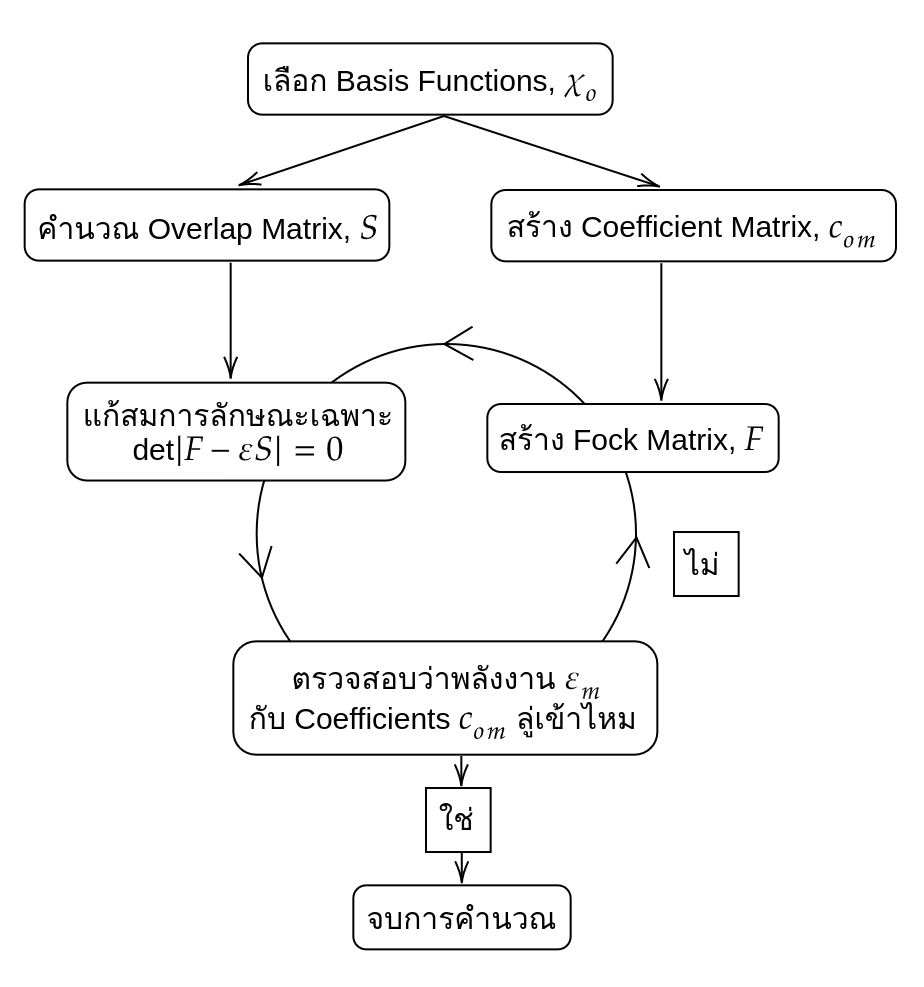
\includegraphics[width=0.8\linewidth]{fig/scf.png}
    \caption{แผนผังขั้นตอนของ SCF ในการประมาณค่าหาพลังงานของออร์บิทัล}
    \label{fig:scf}
\end{figure}

ภาพที่ \ref{fig:scf} แสดงแผนผงอัลกอริทึมของวิธี SCF โดยเริ่มจากการเลือก Atomic Basis Function ซึ่งถือว่าเป็นองค์ประกอบหลักของ%
การนำไปสร้าง (Formulate) $S$ โดยใช้สมการ \ref{eq:matrix_overlap} กับ $c_{om}$ ซึ่งเราจะใช้วิธีการสร้างค่าเริ่มต้นด้วยวิธี Guess 
ซึ่งมีด้วยกันหลายวิธี เช่น

\begin{enumerate}
    \item \textbf{H{\"u}ckel guess} : ใช้ H{\"u}ckel Orbital\autocite{jensen2017}
    
    \item \textbf{Superposition of Atomic Densities (SAD)} : ใช้ผลรวมของ Atomic Density ในการสร้าง Density Matrix
    
    \item \textbf{Generalized Wolfsberg-Helmholtz (GWH)} : เป็นวิธีการที่อาศัย H{\"u}ckel Theory โดยการใช้ Overlap 
    Matrix และ Core Hamiltonian\autocite{wolfsberg1952}
    
    \item \textbf{CORE} : ทำการทำ Core Hamiltonian ให้เกิดเมทริกซ์รูปทแยง (Diagonalization)
    
    \item \textbf{Harris} : ใช้ Harris Functional ซึ่งเป็น Non-self-consistent Approximation สำหรับ Kohn-Sham 
    Orbital\autocite{harris1985}
\end{enumerate}

ซึ่งโปรแกรมเคมีเชิงคำนวณต่างก็มีการเลือกใช้ Guess Method สำหรับการเดา Coefficient หรือ Wavefunction เริ่มต้นในการแก้ SCF แตกต่างกันไป
โปรแกรม Gaussian ใช้วิธี Harris สำหรับการคำนวณ HF และ DFT และใช้ H{\"u}ckel หรือ CORE สำหรับ Semiempirical Methods, 
โปรแกรม Q-Chem และ Psi4 ใช้วิธี SAD กับ GWH เป็นวิธีเริ่มต้นโดยอัตโนมัติ เป็นต้น

หลังจากสร้าง Coefficient Matrix ขั้นตอนต่อไปคือการสร้าง Fock Matrix $F$ โดยใช้สมการ \ref{eq:matrix_fock} 
หลังจากนั้นเราจะทำการแก้สมการลักษณะเฉพาะ (Secular Equation) สมการที่ \ref{eq:scf_secular} เพื่อหา Energy Matrix 
แล้วก็ทำการวนซ้ำขั้นตอนการสร้าง $S$ กับ $F$ ไปปรับหาค่าพลังงานไปเรื่อย ๆ จนกว่าค่าความคลาดเคลื่อนหรือ Error จะมีค่าน้อยกว่าค่าที่กำหนดไว้ 
(Threshold) แล้วจึงสิ้นสุดกระบวนการ SCF เมื่อค่าพลังงานนั้นลู่เข้า

%--------------------------
\subsection{การคำนวณอนุพันธ์ของพลังงานและเมทริกซ์เฮสเซียน}
\label{ssec:ener_der}
\idxen{Energy Derivative}
%--------------------------

หลังจากที่เราสามารถหาพลังงานเชิงอิเล็กทรอนิกส์ (Electronic Energy) ได้แล้ว ลำดับถัดไปที่เราสามารถคำนวณได้ก็คือคุณสมบัติต่าง ๆ ของโมเลกุล
สิ่งแรกที่เราทำได้และถือว่าสำคัญมาก ๆ ในงานวิจัยทางด้านเคมีควอนตัมก็คือการหาโครงสร้างที่เหมาะสมหรือเสถียรที่สุดของโมเลกุลโดยใช้หลักเกณฑ์%
พลังงานรวมที่ต่ำที่สุด ซึ่งการที่เราทราบโครงสร้างที่เหมาะสมที่สุดนั้นมีประโยชน์อย่างมากเพราะเราสามารถนำผลการคำนวณไปเทียบกับผลจากการทดลอง%
ด้วยเทคนิค X-ray Crystallography, Electron Diffractiom, หรือ Microwave Spectroscopy เป็นต้น โดยการหาโครงสร้างที่สภาวะ%
เหมาะสมหรือสมดุล (Equilibrium Structure) นั้นสามารถทำได้โดยหาอนุพันธ์ของพลังงานศักย์ของโมเลกุลเทียบกับพิกัดนิวเคลียร์ ซึ่งวิธีการที่%
เราสามารถนำมาหาอนุพันธ์เพื่อให้ได้ผลลัพเชิงวิเคราะห์ (Analytical Method) เรียกว่า Gradient Method ซึ่งเร็วและให้ผลลัพธ์ที่แม่นยำกว่า%
ระเบียบวิธีเชิงตัวเลข (Numerical Method)

สำหรับอนุพันธ์ของพลังงานนั้นเราจะเริ่มต้นพิจารณากรณีที่ง่าย ๆ นั่นก็คือโมเลกุลที่มีอะตอมสองอะตอม ซึ่งพลังงานศักย์ของโมเลกุลซึ่งเขียนแทนด้วย $E$ 
นี้จะมีเทอมที่เป็นแรงผลักระหว่างนิวเคลียสด้วยซึ่งจะขึ้นกับระยะห่างระหว่างนิวเคลียส (Internuclear Distance, $R$) สำหรับโครงสร้างที่อยู่ในสมดุลนั้น 
แรง (Force) ที่กระทำต่อนิวเคลียสโดยอิเล็กตรอนนั้นจะเท่ากับศูนย์ ซึ่งแรงดังกล่าวเป็นแรงย่อยมีนิยามคืออนุพันธ์อันดับที่หนึ่งของพลังงานศักย์เทียบ%
กับพิกัดของนิวเคลียสที่ $i$

\begin{align}
    f_{i} &= - \pdv{E}{q_{i}} \\
    &= 0
\end{align}

โดยการคำนวณหาอนุพันธ์ข้างต้นด้วยวิธีการวิเคราะห์หรือ Analytical Method นั้นเราจะต้องทำการคำนวณหาอนุพันธ์ของอินทิกรัลของอิเล็กตรอน%
หนึ่งตัวและอิเล็กตรอนสองตัว (One-electron กับ Two-electron Integrals) เทียบกับพิกัดนิวเคลียร์ นั่นคือเราจะต้องทำการหาอนุพันธ์ของ 
Basis Function นั่นเอง\footnote{Basis Function ก็คือ Basis ที่เกิดขึ้นมาจาก Atomic Orbtials ที่ถูก centered หรือมีตำแหน่ง%
อยู่ที่จุดอ้างอิงของนิวเคลียสของอะตอมในโมเลกุล} ซึ่งเราสามารถทำได้ผ่านการใช้กฎลูกโซ่ (Chain Rule) โดยทำการหาอนุพันธ์ของพลังงานศักย์%
เทียบกับ Expansion Coefficient

ลำดับถัดมาคือการหาเมทริกซ์เฮสเซียน (Hessian Matrix) ซึ่งสามารถทำได้โดยการหาอนุพันธ์ย่อยอันดับที่สองของพลังงานศักย์เทียบกับนิวเคลียส%
ของอะตอมตัวที่ $i$ และ $j$ ($\pdv{E}{q_{i}}{q_{j}}$) ซึ่งช่วยให้เราสามารถระบุได้ว่าค่าพลังงานที่คำนวณออกมาได้นั้นสอดคล้องกับ%
จุดต่ำสุดหรือสูงสุดบนพื้นผิวพลังงานศักย์ (Potential Energy Surface หรือ PES) โดยจะสอดคล้องกับอนุพันธ์อันดับที่สองที่ได้ค่าออกมาเป็นบวก 
(สำหรับ Minimum Point) และลบ (สำหรับ Maximum Point) ตามลำดับ

%--------------------------
\section{ทฤษฎีฟังก์ชันนอลความหนาแน่น}
\label{sec:dft}
\idxboth{ทฤษฎีฟังก์ชันนอลความหนาแน่น}{Density Functional Theory}
%--------------------------

ตามที่ผู้เขียนได้พูดถึง \textit{\enquote{ทฤษฎีฟังก์ชันนอลความหนาแน่น}} หรือ \textit{\enquote{Density Functional Theory 
(DFT)}} ในบทก่อนหน้านี้แล้วว่าเป็นทฤษฎีที่มีความสำคัญมากในวงการวิทยาศาสตร์ นั่นก็เพราะว่าเป็นทฤษฎีที่ได้พลิกโฉมงานวิจัยที่เกี่ยวกับกับการ%
ศึกษาโครงสร้างเชิงอิเล็กทรอนิกส์ (Electronic Structure) ของโมเลกุลไปอย่างสิ้นเชิง นั่นก็เพราะว่าแทนที่จะใช้ Wavefunction ในการอธิบาย%
โมเลกุลตรง ๆ วิธี DFT นั้นจะมองโมเลกุลว่าเป็นกลุ่มก้อนของอิเล็กตรอนที่อธิบายโดยใช้ความหนาแน่น ทำให้เราไม่จำเป็นที่จะต้องแก้สมการเพื่อหา 
Wavefunction (ซึ่งไม่มีใครรู้ว่าหน้าตาที่แท้จริงของระบบที่มีมากกว่าหนึ่งอิเล็กตรอนนั้นเป็นอย่างไร)

%--------------------------
\section{ความหนาแน่นเชิงประจุและเมทริกซ์ความหนาแน่น}
\label{sec:charge_den}
\idxboth{ความหนาแน่นเชิงประจุ}{Charge Density}
%--------------------------

ความหนาแน่นเชิงประจุ (Charge Density) เป็นปริมาณที่บ่งบอกถึงประจุของอะตอมที่อยู่ในโมเลกุล ถ้าหากเราทำการอินทิเกรต Charge Density 
ทั่วทั้งปริมาตรเราจะได้ผลลัพธ์เป็นจำนวนของอิเล็กตรอนในระบบของเรา (โมเลกุล) ดังนี้\autocite{szabo1996}

\begin{equation}
    N = \int \rho (\mathbf{r}) dV
\end{equation}

โดยนิยามของ Charge Density จะเป็นผลรวมของโอกาสที่เราจะพบอิเล็กตรอนที่อยู่ภายใน Molecular Orbitals ของทั้งระบบ ดังนี้
\idxen{Charge Density}

\begin{equation}\label{eq:charge_density}
    \rho (\mathbf{r}) = 2 \sum^{N/2}_{i=1} \int |\varphi_{i}(\mathbf{r})|^{2}
\end{equation}

\noindent โดยเลข 2 ด้านหน้าเครื่องหมาย Summation ก็คือ Occupation Number สำหรับกรณีที่ Molecular Orbital ($i$) 
นั้นมีอิเล็กตรอนทั้งแบบ Spin Up และ Spin Down และ $\varphi_{i}(\mathbf{r})$ คือ Wavefunction ซึ่งเราสามารถเขียน Wavefunction 
ให้อยู่ในรูปผลรวมเชิงเส้น (LCAO) ของ Basis Function ($\phi_{i}$) ซึ่ง Basis Function นี้จะเป็นฟังก์ชันอะไรก็ได้ที่สามารถอธิบายการ%
มีอยู่ของ Molecular Orbital โดยในกรณีแบบที่ง่ายที่สุดคือเราจะมองว่า Molecular Orbital นั้นเกิดขึ้นจากการรวมกันของ Atomic Orbitals 
ดังนั้นเราจะกำหนดให้ Atomic Orbitals เป็น Basis Function\footnote{Basis Function ในที่นี้คือ Atomic Orbitals ที่ถูกกำหนดให้%
มีจุดศูนย์กลางอยู่ที่อะตอมนั้น ๆ} ดังนั้นเราสามารถเขียน LCAO ได้ดังต่อไปนี้ 
ตามสมการดังต่อไปนี้
\idxen{Basis Function}

\begin{equation}
    \rho (\mathbf{r}) = 2 \sum_{i} \big( \sum_{\mu} c_{\mu i} \phi_{\mu}^{*} \big) 
    \big( \sum_{\nu} c^{*}_{\nu i}  \phi_{\nu} \big)
\end{equation}

\noindent โดยที่ $c$ คือสัมประสิทธิ์ของ LCAO ลำดับต่อมาคือเมื่อเราจัดรูปให้มีเทอมที่เป็นผลคูณของ Basis Function ($\phi_{\mu}^{*} 
\phi_{\nu}$) เราจะกำหนดให้เทอมนี้เป็นสิ่งที่เรียกว่าเมทริกซ์ซ้อนทับ (Overlap Matrix) ($S_{\mu\nu}$) โดยจะได้สมการที่จัดรูปแล้ว ดังนี้
\idxboth{เมทริกซ์ซ้อนทับ}{Overlap Matrix}

\begin{equation}
    \rho (\mathbf{r}) = 2 \sum_{i}\sum_{\mu\nu} c_{\mu i} c^{*}_{\nu i} S_{\mu\nu}
\end{equation}

หลังจากนั้นเราจะพบว่าจะมีเทอมที่เป็นผลคูณระหว่าง $c$ ซึ่งเราจะกำหนดให้ผลคูณแบบนี้เรียกว่าเมทริกซ์ความหนาแน่น (Density Matrix)
($P_{\mu\nu} = c_{\mu i} c^{*}_{\nu i}$) ซึ่งเราจะได้สมการดังต่อไปนี้
\idxboth{เมทริกซ์ความหนาแน่น}{Density Matrix}

\begin{equation}\label{eq:density_matrix}
    \rho (\mathbf{r}) = 2 \sum_{i} \sum_{\mu\nu} P_{\mu\nu}S_{\mu\nu}
\end{equation}

%--------------------------
\section{ประจุย่อย}
\label{sec:partial_charge}
\idxboth{ประจุย่อย}{Partial Charge}
%--------------------------

การวิเคราะห์ Wavefunction หลังจากการคำนวณเป็นสิ่งที่สำคัญมากเพราะจะช่วยให้เราเข้าใจถึงพฤติกรรมเชิงอิเล็กทรอนิกส์ของอะตอมภายในโมเลกุล 
โดยสิ่งที่นักเคมีทฤษฎีมักจะทำการวิเคราะห์เป็นอันดับแรกเสมอนั่นก็คือประจุย่อยของแต่ละอะตอม (Partial Atomic Charge) คำถามคือ 
ทำไมประจุย่อยถึงมีความสำคัญ? คำตอบคือถ้าหากเราทราบถึงประจุย่อยของโมเลกุลแล้วนั้นจะช่วยทำให้สามารถเข้าใจว่าอะตอมแต่ละตัวส่งผลหรือมี 
Contribution มากน้อยเพียงใดเมื่อเทียบกับอะตอมอื่น ๆ ภายในโมเลกุลเดียวกัน

%--------------------------
\section{พลังงานของ Frontier Orbitals}
\label{sec:ener_orb}
%--------------------------

\idxen{Frontier Orbitals}

\idxen{Ground State}

%--------------------------
\subsection{พลังงานของ HOMO และ LUMO}
\label{ssec:ener_homo_lumo}
\idxth{พลังงานของ HOMO และ LUMO}
%--------------------------

\idxen{Frontier Orbitals!HOMO}

\idxen{Frontier Orbitals!LUMO}

%--------------------------
\subsection{ผลต่างของพลังงานของ HOMO และ LUMO}
\label{sec:ener_diff_orb}
%--------------------------

\idxen{Energy Gap}

%--------------------------
\section{พื้นผิวพลังงานศักย์}
\label{sec:pef}
\idxboth{พื้นผิวพลังงานศักย์}{Potential Energy Surface}
%--------------------------

หนึ่งในหัวข้อที่สำคัญของเคมีเชิงคำนวณก็คือพื้นผิวพลังงานศักย์ (Potential Energy Surface) ซึ่งเป็นสิ่งที่อธิบายความสัมพันธ์ระหว่างรูปร่างเชิง%
เรขาคณิตของโมเลกุล (Molecular Geometry) เช่น ตำแหน่งที่สัมพันธ์กันของอะตอมในโมเลกุลและพลังงานเชิงโมเลกุล พื้นผิวพลังงานศักย์ที่เรา%
จะมาศึกษากันในบทนี้จะเป็นพื้นผิวแบบง่ายสำหรับโมเลกุลเล็ก ๆ เช่น โมเลกุลอะตอมคู่ (Diatomic Molecular) และ โมเลกุลที่มีสามอะตอม 
เพื่อให้ง่ายต่อการอ่านและเพื่อความกระชับ ผู้เขียนจะขอใช้ตัวย่อ PES ซึ่งย่อมาจาก Potential Energy Surface แทนการเรียกพื้นผิวพลังงานศักย์%
ซึ่งจะยาวเกินไป

%--------------------------
\subsection{พื้นผิวพลังงานศักย์สำหรับโมเลกุลอะตอมคู่}
\label{ssec:pef_di_atomic}
%--------------------------

โดยทั่วไปแล้ว PES สำหรับระบบที่ประกอบไปด้วยอะตอมหลายอะตอมนั้นจริง ๆ แล้วก็เป็นฟังก์ชันหลายมิติเชิงซ้อนแบบหนึ่ง ซึ่งเรียกเป็นภาษาอังกฤษว่า
Complex Multidimensional Function ตัวอย่างเช่นเรามีระบบ (โมเลกุล) ที่มีอะตอม $N$ อะตอม ความสัมพันธ์ระหว่างอะตอมภายในระบบนี้%
สามารถถูกอธิบายได้ด้วย Degree of Freedom ซึ่งมีจำนวนเท่ากับ $3N-6$ สำหรับกรณีโมเลกุลที่ไม่เป็นเชิงเส้น เช่น โมเลกุลน้ำ (\ce{H2O}) 
และมีจำนวนเท่ากับ $3N-5$ สำหรับกรณีที่โมเลกุลเป็นแบบเชิงเส้น เช่น โมเลกุลแก๊สคาร์บอนไดออกไซด์ (\ce{CO2}) ซึ่งการที่ฟังก์ชัน Degree 
of Freedom มีจำนวนมิติที่มากเกินกว่า 3 มิตินี้ ทำให้ยากต่อมิงและวิเคราะห์ PES ดังนั้นวิธีที่ง่ายที่สุดคือเรามักจะทำการพิจารณาเฉพาะ Degree of 
Freedom ที่สำคัญและเกี่ยวข้องกับการเปลี่ยนเปลี่ยนของระบบและพลังงาน โดยที่เราเรียกพารามิเตอร์ที่เราทำการเปลี่ยนค่าไปเรื่อย ๆ เพื่อดูผลต่อการ%
เปลี่ยนแปลงพลังงานของโมเลกุลนี้ว่าพิกัดของปฏิกิริยา (Reaction Coordinates) 

เรามาเริ่มกันด้วยตัวอย่างแรกด้วย PES ของอะตอมคู่ ดังต่อไปนี้

\begin{figure}[H]
    \centering
    \begin{subfigure}{0.5\textwidth}
        \centering
        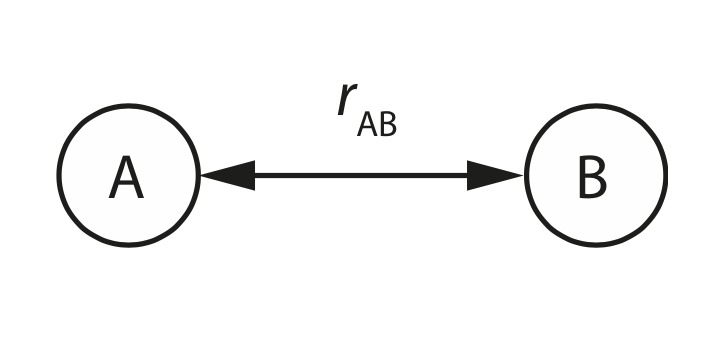
\includegraphics[width=0.9\linewidth]{fig/diatomic_molecule.png}
        \caption{กำหนดระยะห่างระหว่างอะตอม}
        \label{fig:diatomic_mol}
    \end{subfigure}%
    \begin{subfigure}{0.5\textwidth}
        \centering
        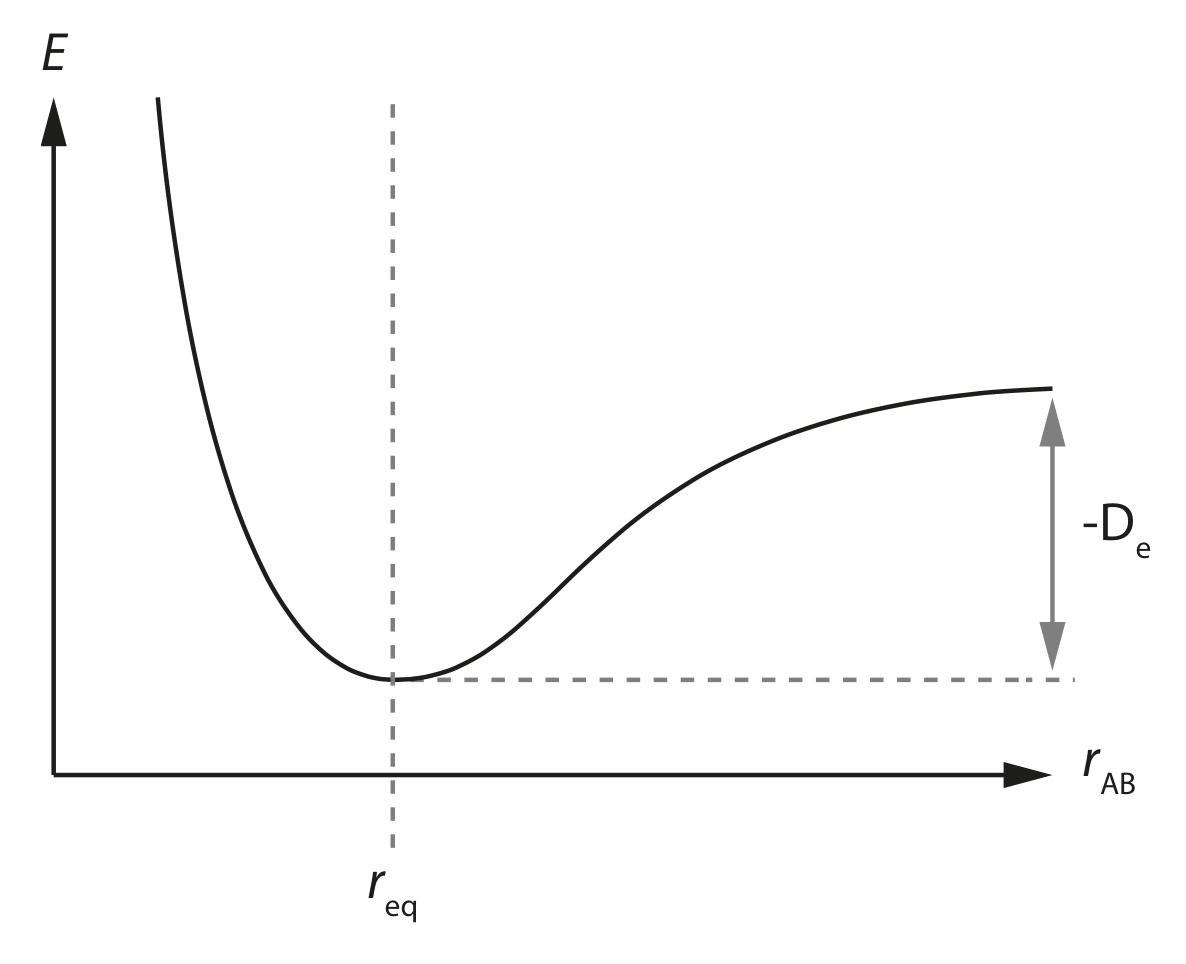
\includegraphics[width=0.9\linewidth]{fig/PES_diatomic_mol.png}
        \caption{พลังงานศักย์ของโมเลกุลคู่}
        \label{fig:PES_diatomic}
    \end{subfigure}
    \caption{โมเลกุลคู่}
    \label{fig:diatomic_mol_and_PES}
\end{figure}

สำหรับคู่อะตอม A และ B มี Degree of Freedom เพียงแค่ 1 Degree เท่านั้น และกำหนดให้ระยะห่างระหว่างอะตอมเป็น $r_{AB}$ ถ้าอะตอม 
A มีการสร้างพันธะกับอะตอม B สิ่งที่เกิดขึ้นคือเรา(อาจจะ)สามารถทำนายลักษณะของ PES ของโมเลกุลนี้ได้ ดังต่อไปนี้

\begin{figure}[H]
    \centering
    \begin{subfigure}{0.5\textwidth}
        \centering
        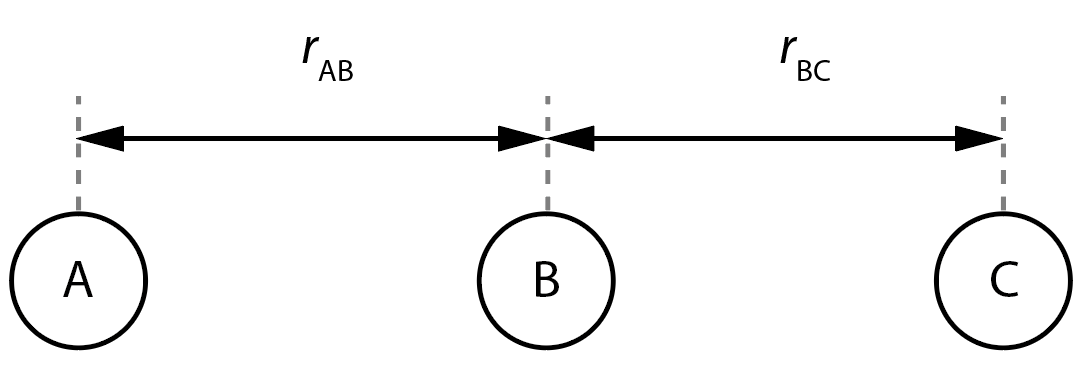
\includegraphics[width=0.9\linewidth]{fig/3-body_collinear.png}
        \caption{กำหนดระยะห่างระหว่างอะตอม}
        \label{fig:3_body_mol}
    \end{subfigure}%
    \begin{subfigure}{0.5\textwidth}
        \centering
        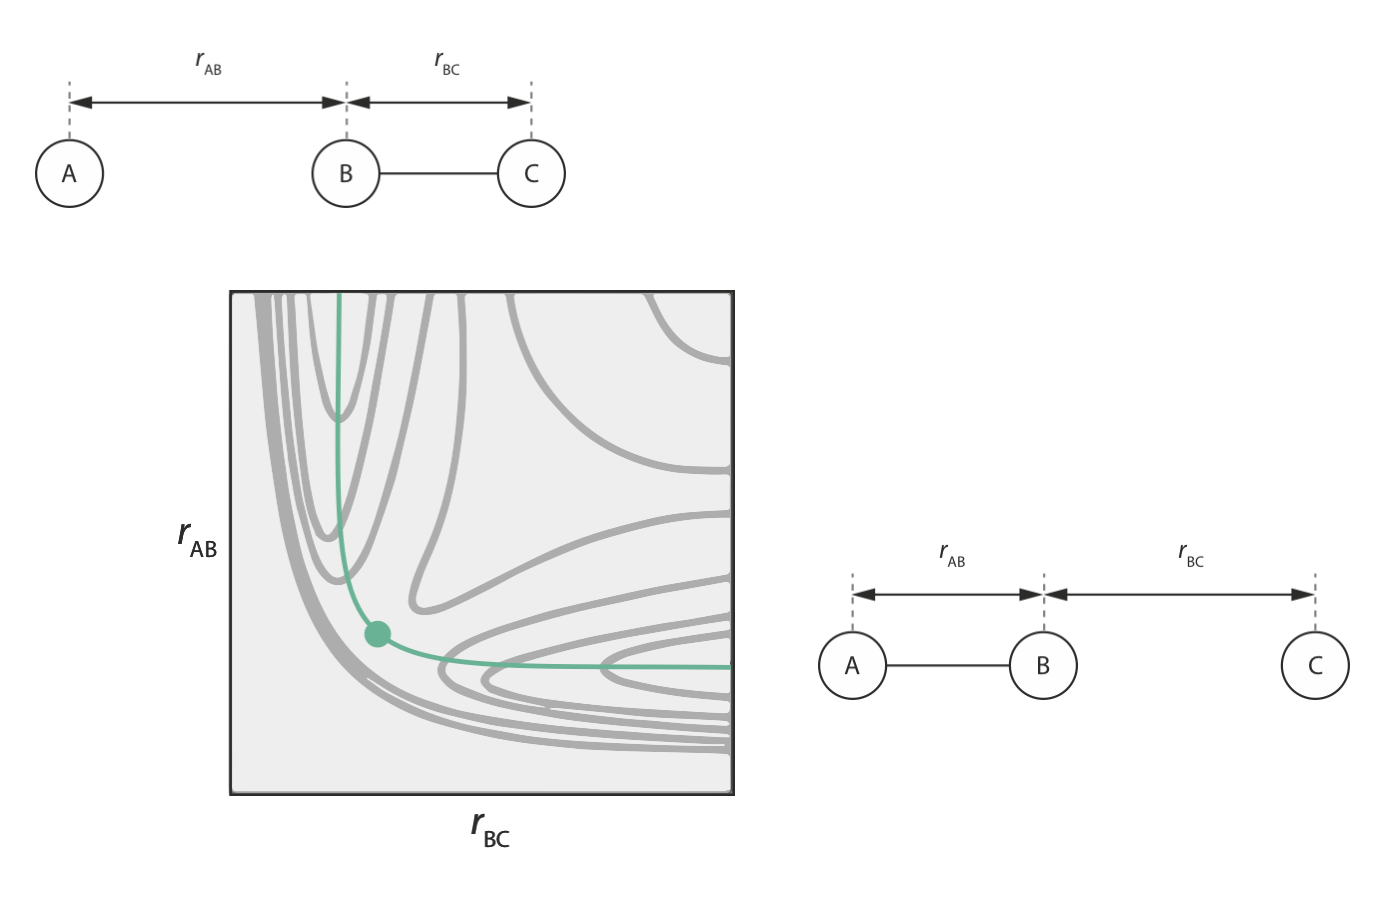
\includegraphics[width=0.9\linewidth]{fig/3-body_collinear_PES.png}
        \caption{พลังงานศักย์ของโมเลกุลสามอะตอมแบบเชิงเส้นตรงร่วม}
        \label{fig:PES_3_body_mol}
    \end{subfigure}
    \label{fig:3_body_mol_and_PES}
\end{figure}

\begin{figure}[H]
    \centering
    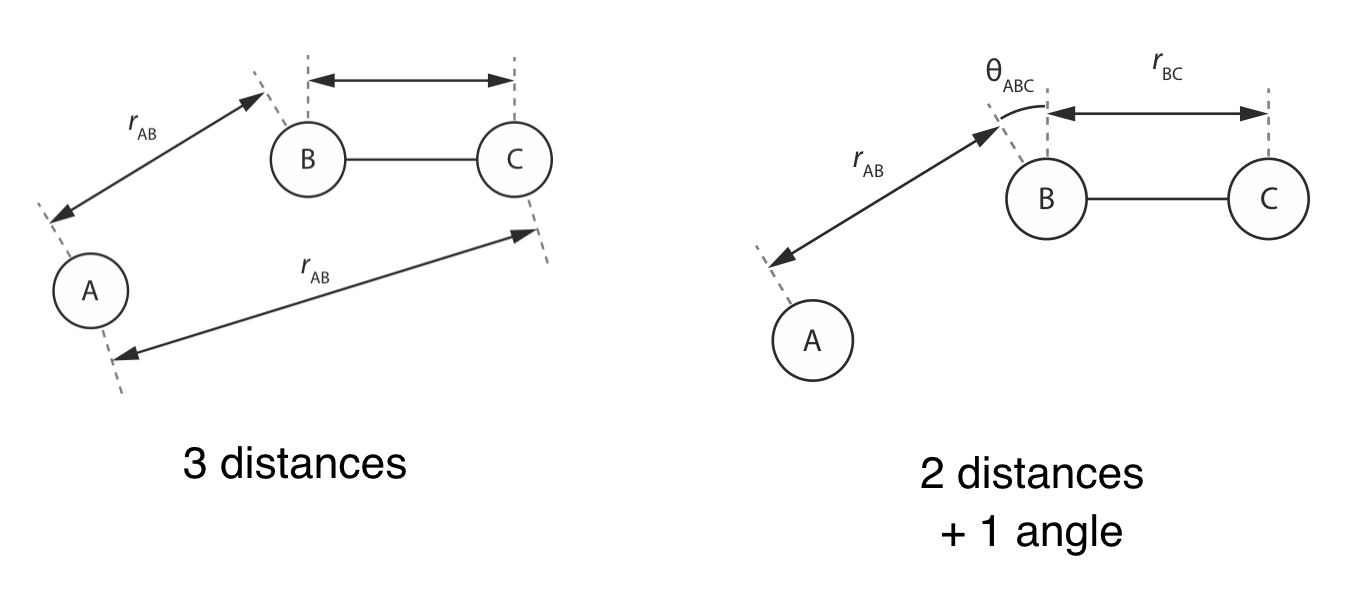
\includegraphics[width=0.8\linewidth]{fig/3-body_non-collinear.png}
    \caption{โมเลกุลสามอะตอมแบบไม่เป็นเชิงเส้นตรงร่วม}
    \label{fig:non_collinear}
\end{figure}

\begin{figure}[H]
    \centering
    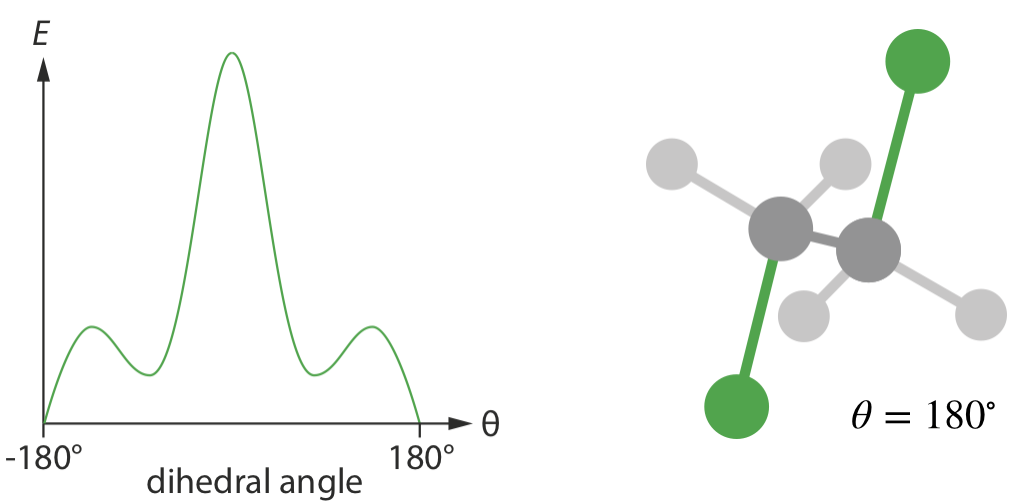
\includegraphics[width=0.8\linewidth]{fig/PES_C2H4Cl2.png}
    \caption{พลังงานศักย์ของโมเลกุล \ce{C22H4Cl2}}
    \label{fig:pes_c2h4cl2}
\end{figure}

%--------------------------
\section{ไดโพลโมเมนต์}
\label{sec:dipole_moment}
%--------------------------

ไดโพลโมเมนต์ (Dipole Moment)

\idxen{Dipole Moment}

%--------------------------
\section{สภาพการเกิดขั้ว}
\label{sec:polariz}
%--------------------------

สภาพการเกิดขั้ว (Polarizability)
\idxen{Polarizability}

%--------------------------
\section{เทคนิคสเปกโทรสโกปีแบบสั่น}
\label{sec:spectro}
\idxen{Spectroscopy}
\idxen{Spectroscopy!Vibrational Spectroscopy}
%--------------------------

สเปกโทรสโกปี (Spectroscopy) เป็นการศึกษาอันตรกิริยา (Interaction) ระหว่างสสารกับรังสีแม่เหล็กไฟฟ้า (Electromagnetic Radiation) 
ที่เกิดจากการเปลี่ยนระดับพลังงานของอิเล็คตรอน การเปลี่ยนระดับพลังงานการหมุน (Rotation) และการสั่นสะเทือน (Vibration) ของโมเลกุล 
ซึ่งการที่เราทราบจากสเปกตรัมของโมเลกุลจะทำให้เราทราบข้อมูลหลายอย่างเกี่ยวกับโครงสร้างของโมเลกุลของสสารและสมบัติทางเคมี เช่น

\begin{itemize}
    \item สมมาตรของโมเลกุล (Symmetry)
    
    \item ความยาวพันธะ (Bond Length)
    
    \item มุมพันธะ (Bond Angle)
    
    \item ความแข็งแรงของพันธะ (Bond Strength)
    
    \item การเปลี่ยนแปลงภายในและระหว่างโมเลกุล
\end{itemize}

\noindent โดยในหัวข้อนี้เราจะมาดูรายละเอียดเกี่ยวกับการคำนวณความเข้มของการดูดกลืนสำหรับเทคนิค Infrared (IR) และรามาน (Raman) 
ซึ่งทั้งสองเทคนิคนี้ต่างก็เป็นเทคนิคสเปกโทรสโกปีแบบสั่น (Vibrational Spectroscopy) ซึ่งมีการนำมาใช้ในการทำงานวิจัยสำหรับการศึกษา%
คุณสมบัติของโมเลกุลอย่างแพร่หลาย

%--------------------------
\subsection{อินฟาเรดสเปกโทรสโกปี}
\label{ssec:ir_spectro}
\idxboth{สเปกโทรสโกปี!อินฟาเรด}{Spectroscopy!IR}
%--------------------------

อินฟาเรดสเปกโทรสโกปี (IR Spectroscopy) เป็นการวัดการดูดกลืนของการแผ่รังสีของโมเลกุลในช่วงอินฟราเรดซึ่งเกี่ยวข้องกับการเปลี่ยนแปลงของ%
อิเล็กทริกไดโพลโมเมนต์ (Electric Dipole Moment) ของโมเลกุลที่ศึกษา สำหรับการคำนวณความเข้มของการดูดกลืน IR ในรูปแบบของวิธีแบบ
Dynamic นั้นสามารถทำได้โดยใช้สมการ (ความสมพันธ์) ดังต่อไปนี้s\autocite{thomas2013}

\begin{equation}\label{eq:IR_corr}
    I_{IR} (\omega) \propto \int \braket{\bm{\dot{\mu}}(\tau) \bm{\dot{\mu}}(\tau+t)}_{\tau} e^{-i \omega t} dt
\end{equation}

\noindent โดยที่ $\bm{\dot{\mu}}$ คืออนุพันธ์ของไดโพลโมเมนต์เทียบกับเวลา, $\omega$ คือความถี่เชิงการสั่น (Vibrational Frequency),
$\tau$ คือเวลาที่เปลี่ยนแปลงไปอย่างช้า ๆ และ $t$ คือเวลาสำหรับการทำ Integration นอกจากนี้ยังจะสังเกตได้ว่าจะมีเทอม
$\braket{\bm{\dot{\mu}}(\tau) \bm{\dot{\mu}}(\tau+t)}_{\tau}$ ซึ่งจะเป็นตัวที่บ่งบอกถึงสหสัมพันธ์ของเวลา (Time Correlation) 
ของ $\bm{\dot{\mu}}$ 

สำหรับกรณีที่เป็นแบบ Static นั้น สเปกตรัทของ IR สามารถคำนวณได้ผ่านอนุพันธ์ของไดโพลโมเมนต์เทียบกับพิกัดหรือตำแหน่งของโหมดการสั่น%
แบบปกติ (Normal Coordinates) ซึ่งจะไม่ขึ้นกับเวลา ด้วยสมการดังต่อไปนี้

\begin{equation}\label{eq:mu_qm}
    \bm{\mu}= \sum_{\mu\nu} P_{\mu\nu} \braket{\phi_{\mu}|\bm{r}|\phi_{\nu}}
\end{equation}

\begin{equation}\label{eq:mu_classical}
    \bm{\mu}=\sum_{J} q_J \bm{R_J}
\end{equation}

โดยที่สมการ \ref{eq:mu_qm} จะเป็นสำหรับกรณีแบบควอนตัมซึ่งจะคำนวณผ่านเมทริกซ์ความหนาแน่นและ Basis Function แต่สมการ 
\ref{eq:mu_classical} จะเป็นสำหรับกรณีแบบดั้งเดิมซึ่งจะคำนวณผ่านจุดประจุ (Point Charge) และพิกัดคาร์ทีเซียนของอะตอม

%--------------------------
\subsection{รามานสเปกโทรสโกปี}
\label{ssec:raman_spectro}
\idxboth{สเปกโทรสโกปี!รามาน}{Spectroscopy!Raman}
%--------------------------

รามานสเปกโทรสโกปี (Raman Spectroscopy) เป็นเทคนิคหนึ่งที่เปรียบเมือนเป็นพี่น้องกับเทคนิคอินฟาเรดสเปกโทรสโกปี โดยที่ Raman Spectroscopy 
จะเป็นผลมาจากการเกิดการกระเจิงของแสงแบบไม่ยืดหยุ่นในช่วงอินฟราเรด วิสิเบิล (Visible) และอัลตราไวโอเล็ต (Ultraviolet) ซึ่งเกี่ยวข้อง%
กับการเปลี่ยนแปลงสภาพการเกิดขั้ว (Polarizability) แบบอิเล็กทริกไดโพล-อิเล็กทริกไดโพล (Electric-dipole--electric-dipole) 
ของสสาร โดยความเข้มของการกระเจิงแบบรามาน ($I_{Raman}$) สามารถคำนวณได้ด้วยความสัมพันธ์ดังต่อไปนี้\autocite{thomas2013}

\begin{equation}\label{eq:Raman_corr}
    I_{Raman} (\omega) \propto \frac{(\omega_{in}-\omega)^4}{\omega} 
    \frac{1}{1-\exp(-\frac{\hbar\omega}{k_{B}T})}S(a^{2}, \gamma^{2})
\end{equation}

\noindent โดยที่ $S(a^{2}, \gamma^{2})$ คือตัวแปรที่เป็นผลจากการรวมกันของความคงที่ (ไม่เปลี่ยนแปลง) แบบไอโซโทรปิค (Isotropic) 
และแอนิโซโทรปิค (Anisotropic)\footnote{คำจำกัดความ: คุณสมบัติที่เท่ากันทุกทิศทาง (Isotropic) และคุณสมบัติที่ขึ้นอยู่กับทิศทาง 
(Anisotropic)} ของเทนเซอร์แบบ Placzek-type Polarizability ($\bm{\alpha}$)\autocite{jensen2005}, $\omega$ 
คือความถี่เชิงการสั่น, $\omega_{in}$ คือความถี่ของแสดง, $k_{B}$ คือค่าคงที่ของโบลทซ์มานน์ (Boltzmann Constant) และ $T$ 
คืออุณหภูมิของระบบในหน่วย Kelvin โดยสมการที่จะใช้ในการอธิบาย $S(a^{2}, \gamma^{2})$ จะขึ้นอยู่กับรูปแบบของการทดลองและสมการของ 
Time Correlation\autocite{mattiat2021}

%--------------------------
\section{การถ่ายโอนอิเล็กตรอน}
\label{sec:et}
\idxth{การถ่ายโอนอิเล็กตรอน}
\idxen{Electron Transfer}
%--------------------------

การถ่ายโอนอิเล็กตรอน (Electron Transfer) เป็นกระบวนการที่อิเล็กตรอนเปลี่ยนตำแหน่งหรือเคลื่อนย้ายจากอะตอมหนึ่งไปยังอีกอะตอมหนึ่ง 
(Transfering) โดยเราสามารถแบ่งการถ่ายโอนอิเล็กตรอนออกได้เป็นสองกรณีคือการถ่ายโอนระหว่างโมเลกุล (Intermolecular Electron 
Transfer) และการถ่ายโอนภายในโมเลกุล (Intramolecular Electron Transfer) สำหรับการถ่ายโอนกรณีแรกนั้นมีสิ่งเร้าภายนอกเป็นปัจจัยหลัก 
ตัวทำละลายหรือสิ่งแวดล้อมภายนอกเป็นตัวกระตุ้นหรือตัวขับเคลื่อน (Driving Force) ที่ทำให้เกิดการถ่ายโอนจากโมเลกุลหนึ่งไปยังโมเลกุลหนึ่ง
สำหรับการถ่ายโอนกรณีที่สองนั้นจริง ๆ แล้วมีปัจจัยหลายอย่างที่ทำให้เกิดกระบวนการนี้ เช่น ความเสถียรเชิงโครงสร้างของโมเลกุล (Stability) 
ซึ่งเกิดจากการรบกวนจากภายนอกที่ส่งผลให้โครงสร้างเชิงอิเล็กทรอนิกส์ของโมเลกุลเปลี่ยนไป 

ในการพิจารณาการถ่ายโอนอิเล็กตรอนทั้งสองกรณีนี้สามารถอธิบายได้ดังนี้ ให้ผู้อ่านลองจินตนาการมีกล่องอยู่สองกล่อง โดยกล่องซ้ายใส่ลูกบอลไว้ 
ส่วนกล่องขวานั้นว่างเปล่า หลังจากนั้นเราทำการหยิบลูกบอลจากกล่องซ้ายแล้วนำไปใส่ไว้ในกล่องขวา นี่คือเป็นการจำลองการถ่ายโอนอิเล็กตรอน 
จากเหตุการณ์ดังกล่าวเราแบ่งออกได้เป็นสองเหตุการณ์ย่อยคือ

\begin{enumerate}
    \item เหตุการณ์ที่เกิดขึ้นก่อนที่จะเกิดการถ่ายโอนอิเล็กตรอน
    
    \item เหตุการณ์ที่เกิดหลังจากถ่ายโอนอิเล็กตรอนแล้ว
\end{enumerate}

\begin{figure}[H]
    \centering
    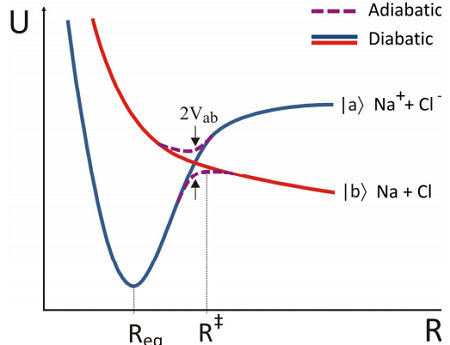
\includegraphics[width=0.7\linewidth]{fig/et_diagram.png}
    \caption{แผนภาพแสดงพื้นผิวพลังงานศักย์ของกระบวนการถ่ายโอนอิเล็กตรอน (เครดิตภาพ: \url{https://chem.libretexts.org})}
    \label{fig:et_diagram}
\end{figure}

%--------------------------
\subsection{ค่าคู่ควบของการถ่ายโอนอิเล็กตรอน}
\label{ssec:et_coupling}
\idxth{การถ่ายโอนอิเล็กตรอน!ค่าคู่ควบ}
\idxen{Electron Transfer!Electron Transfer Coupling}
%--------------------------

ค่าคู่ควบของการถ่ายโอนอิเล็กตรอน (Electron Transfer Coupling) เป็นค่าคู่ควบที่เกิดขึ้นจากการถ่ายโอนอิเล็กตรอน

%--------------------------
\subsection{พลังงานการปรับเปลี่ยนโครงสร้าง}
\label{ssec:reor_ener}
\idxth{พลังงานการปรับเปลี่ยนโครงสร้าง}
\idxen{Reorganization Energy}
%--------------------------

พลังงานการปรับเปลี่ยนโครงสร้าง (Reorganization Energy) คือพลังงาน(ที่น้อยที่สุด)ที่ใช้ในการปรับเปลี่ยนโครงสร้างของโมเลกุลเพื่อทำให้เกิด%
การถ่ายโอนอิเล็กตรอนได้

%--------------------------
\section{คุณสมบัติของสถานะกระตุ้น}
\label{sec:ex_prop}
\idxth{สถานะกระตุ้น}
\idxen{Excited State}
%--------------------------

คุณสมบัติของอิเล็กตรอน ณ สถานะกระตุ้น (Excited State Properties)
\idxth{สถานะกระตุ้น!คุณสมบัติของอิเล็กตรอน ณ สถานะกระตุ้น}
\idxen{Excited State Properties}

%--------------------------
\subsection{พลังงานของสถานะกระตุ้น}
\label{ssec:ex_ener}
\idxth{สถานะกระตุ้น!พลังงานของสถานะกระตุ้น}
\idxen{Excited State!Excited State Energies}
%--------------------------

พลังงานของสถานะกระตุ้น (Excited State Energies)

%--------------------------
\subsection{ค่าคู่ควบของกระบวนการนอนอะเดียแบติก}
\label{ssec:nonadia_ener}
\idxth{สถานะกระตุ้น!ค่าคู่ควบแบบนอนอะเดียแบติก}
\idxen{Excited State!Nonadiabatic Coupling}
%--------------------------

ค่าคู่ควบแบบนอนอะเดียแบติก (Nonadiabatic Coupling)
